%----------------------------------------------------------------------------------------
%	PACKAGES AND OTHER DOCUMENT CONFIGURATIONS
%----------------------------------------------------------------------------------------

\documentclass[twoside,onecolumn]{article}
\usepackage[labelfont=bf]{caption} %Makes all label bold
\usepackage{blindtext} % Package to generate dummy text throughout this template 
\usepackage{listings}
\usepackage{amsmath}
\usepackage{graphicx}
\usepackage{mathrsfs}
\usepackage{subfig}
\usepackage{wrapfig}
\usepackage{listings}
\usepackage{float}
\usepackage{subfig}
\usepackage[dvipsnames]{xcolor}
\usepackage[utf8]{inputenc}
\usepackage[sc]{mathpazo} % Use the Palatino font
\usepackage[T1]{fontenc} % Use 8-bit encoding that has 256 glyphs
\linespread{1.2} % Line spacing - Palatino needs more space between lines
\usepackage{microtype} % Slightly tweak font spacing for aesthetics
\usepackage{cite} %Citing references
\usepackage[english]{babel} % Language hyphenation and typographical rules

\usepackage[hmarginratio=1:1,top=32mm,columnsep=20pt]{geometry} % Document margins
%\usepackage[hang, small,labelfont=bf,up,textfont=it,up]{caption} % Custom captions under/above floats in tables or figures
%\usepackage{booktabs} % Horizontal rules in tables
\usepackage{lettrine} % The lettrine is the first enlarged letter at the beginning of the text
%\setlength\belowcaptionskip{-3ex}
\usepackage{enumitem} % Customized lists
\setlist[itemize]{noitemsep} % Make itemize lists more compact

% From Mortens project latex file
\usepackage{bm,ltablex,microtype}

% Write symbols bigger
\usepackage{relsize}

\usepackage{abstract} % Allows abstract customization
\renewcommand{\abstractnamefont}{\normalfont\bfseries} % Set the "Abstract" text to bold
\renewcommand{\abstracttextfont}{\normalfont\small\itshape} % Set the abstract itself to small italic text

\usepackage{titlesec} % Allows customization of titles
\renewcommand\thesection{\Roman{section}} % Roman numerals for the sections
\renewcommand\thesubsection{\roman{subsection}} % roman numerals for subsections
\titleformat{\section}[block]{\large\scshape\centering}{\thesection.}{1em}{} % Change the look of the section titles
\titleformat{\subsection}[block]{\large}{\thesubsection.}{1em}{} % Change the look of the section titles

\usepackage{fancyhdr} % Headers and footers
\pagestyle{fancy} % All pages have headers and footers
\fancyhead{} % Blank out the default header
\fancyfoot{} % Blank out the default footer
\fancyhead[C]{Computational Physics} % Custom header text
\fancyhead[R]{\href{https://github.com/patrykpk/FYS4150/tree/master/Project_2}{Scripts - GitHub}} % Custom header text
\rfoot{\thepage} 
\renewcommand{\footrulewidth}{0.4pt}% Default \footrulewidth is 0pt

\usepackage{titling} % Customizing the title section


\usepackage{hyperref} % For hyperlinks in the PDF
%----------------------------------------------------------------------------------------
%----------------------------------------------------------------------------------------

\graphicspath{{Pictures/}} %Path to pictures
\date{\today} % Leave empty to omit a date


\setlength\parindent{0pt}
%\setlength{\parskip}{0mm}
%\setlength{\textfloatsep}{5pt}
%\setlength{\intextsep}{10mm}
%\renewcommand{\baselinestretch}{1.5}


\begin{document}

%----------------------------------------------------------------------------------------------------------------
%     TITLE PAGE
%----------------------------------------------------------------------------------------------------------------

\begin{titlepage} % Suppresses headers and footers on the title page

	\centering % Centre everything on the title page
	
	\scshape % Use small caps for all text on the title page
	
	\vspace*{\baselineskip} % White space at the top of the page
	
	%------------------------------------------------
	%	Title
	%------------------------------------------------
	
	\rule{\textwidth}{1.6pt}\vspace*{-\baselineskip}\vspace*{2pt} % Thick horizontal rule
	\rule{\textwidth}{0.4pt} % Thin horizontal rule
	
	\vspace{0.75\baselineskip} % Whitespace above the title
	
	{\LARGE Jacobi's method for solving eigenvalue problems \\ %eigenvalue problem schrödinger equation \\
	\bigskip
	FYS4150} % Title
	
	\vspace{0.75\baselineskip} % Whitespace below the title
	
	\rule{\textwidth}{0.4pt}\vspace*{-\baselineskip}\vspace{3.2pt} % Thin horizontal rule
	\rule{\textwidth}{1.6pt} % Thick horizontal rule
	
	\vspace{2\baselineskip} % Whitespace after the title block
	
	%------------------------------------------------
	%	Subtitle
	%------------------------------------------------
	
	%{\LARGE FYS4150 } % Subtitle or further description
	
	\vspace*{3\baselineskip} % Whitespace under the subtitle
	
	%------------------------------------------------
	%	Editor(s)
	%------------------------------------------------
	
    
    \large Written by:
	
	\vspace{0.5\baselineskip} % Whitespace before the editors
	
	\textit{ Marius Enga, Patryk Krzyzaniak\\ Mohamed Ismail and Kristoffer Varslott \\} % Editor list
	
	\vspace{0.5\baselineskip} % Whitespace below the editor list
	
	\bigskip
	
	Department of Physics UiO % Editor affiliation
	
	\bigskip
	\bigskip
	\bigskip
	\bigskip
	\bigskip
	\bigskip
	\bigskip
	\graphicspath{{Pictures/}} %Path to pictures
	
\includegraphics[scale = 0.7]{University.png}
	\vfill % Whitespace between editor names and publisher logo
	
	%------------------------------------------------
	\bigskip
	\bigskip
	
	
	%\textit{\href{http://www.github.com}{Source code GitHub}}% Your email address
	%------------------------------------------------
	\bigskip
	\bigskip
	\bigskip
	\bigskip
	\vspace{0.3\baselineskip} % Whitespace under the publisher logo
	
	\today

\end{titlepage}

%----------------------------------------------------------------------------------------------------------------
%     END TITLE PAGE
%----------------------------------------------------------------------------------------------------------------



% ------------------- main content ----------------------
%----------------------------------------------------------------------------------------------------------------
%     Abstract
%----------------------------------------------------------------------------------------------------------------

\tableofcontents
\newpage
\begin{abstract}
Eigenvalue problems in physics can often be discretized into a linear algebra problem which can be solved by diagonalizing a matrix. Using Jacobi's method to diagonalize, we are able to solve the buckling beam problem and the three-dimensional harmonic oscillator potential with both one and two electrons. We found that Jacobi's method is a brute force method that works good for solving these problems, but it will run slowly for high dimensionality matrices if a high precision in the eigenvalues are desired. Ground state eigenvalues and a couple of the first exited states however are quite accurate, even for low dimensions. 
\end{abstract}
%Altering Listing
\definecolor{mygray}{gray}{0.95}
\lstdefinestyle{customc}{
  belowcaptionskip=1\baselineskip,
  breaklines=true,
  frame=L,
  backgroundcolor=\color{mygray},
  xleftmargin=\parindent,
  language=C++,
  showstringspaces=false,
  basicstyle=\footnotesize\ttfamily,
  keywordstyle=\bfseries\color{green!40!black},
  commentstyle=\itshape\color{purple!40!black},
  identifierstyle=\color{blue},
  stringstyle=\color{orange},
  %doublestyle=\color{red},
}

%----------------------------------------------------------------------------------------------------------------
%     INTRODUTCTION
%----------------------------------------------------------------------------------------------------------------

\section{Introduction}
%se igjennom! kan endre på noe
Solving differential equations is a vital part of physics, where most of the problems encountered is somehow related to differential equations. This article takes a good look at how to solve differential equations by transforming them into eigenvalue problems. \\
In this project we will develop a code for solving eigenvalue problems. Starting of with a classical mechanics problem with a buckling beam case, we then move on to the quantum mechanical realm with a three-dimensional harmonic oscillator potential with both one and two electrons.

\bigskip

By utilizing our eigenvalue solver, we can solve all these problems by changing the diagonal elements of the tridiagonal Toeplitz matrix. In order to use the eigenvalue solver, the equations have to be scaled according to the different cases that will be studied upon.

%To use our general eigenvalue solver, we will need to scale the equations for the different cases we are studying.

Our eigenvalue solver will be implementing the Jacobi's rotation algorithm.


\bigskip

In all the cases we are studying there exists exact analytical solutions for the eigenvalues which we will be comparing our numerical results with. In addition, the implemented eigenvalue solver will be compared to a solver found in the Armadillo\cite{Sanderson2019}\cite{Saddler1971} package with respect to the CPU time. The analytical solutions for the eigenvalues concerning the two electron scenario were obtained by M. Taut \cite{taut}.  

\section{Theory}

\subsection{The buckling beam problem}
%se igjennom! kan endre på noe
We start of with following differential equation: 

\begin{equation*}
\gamma \frac{d^2 u(x)}{dx^2} = -F u(x),
\end{equation*}

\bigskip

This second order differential equation is called "The buckling beam problem", which is a classical wave function problem in one dimension. In the equation above $u(x)$ is the vertical displacement of the beam in the $y$-direction. The beam has length $L$, $x\in [0,L]$ and $F$ is a force applied at $(L,0)$ in the direction towards the origin. The parameter $\gamma$ is a constant defined by properties like the rigidity of the beam. Applying Dirichlet boundary conditions, for then to set $u(0)=u(L)=0$.

\bigskip

In this specific case two of the  parameters $\gamma$, $F$ and $L$ are known. An assumption is made where F and L is known, thereafter by creating a dimensional variable $\rho = \frac{x}{L}$ and inserting it as a function of $u(x)$. The equation can be rewritten as: 

\bigskip

\begin{equation}
 \frac{d^2(\rho)}{d\rho^2} = -\frac{FL^2}{\gamma} u(\rho)=-\lambda u(\rho)
\end{equation}

\bigskip

Where the boundaries is as before: $\rho \in [0,1]$. $\lambda$ is then defined as  $\lambda= FL^2/\gamma$. We need to discretize this equation to obtain the eigenvalues. Writing this second order equation to a discretized form yields: 

\bigskip

\begin{equation}
-\frac{u_{i+1} -2u_i +u_{i-1} }{h^2}  = \lambda u_i.
\label{eq:eq1}
\end{equation}

\bigskip

Where the step-length $h$ as been introduced and can is defined as: 

\bigskip

 \begin{equation*}
  h=\frac{\rho_N-\rho_0 }{N}
\end{equation*}

\bigskip

where $\rho_N$ and $\rho_0$ is 1 and 0 respectively. Then it is valid to define $\rho_i$ as discretized:

\bigskip

 \begin{equation*}
    \rho_i= \rho_0 + ih \hspace{1cm} i=1,2,\dots , N.
\end{equation*}

\bigskip

It is possible to rewrite equation \ref{eq:eq1} as a set of linear equation: 

\bigskip

\begin{equation*}
    \begin{bmatrix} d& a & 0   & 0    & \dots  & 0 \\
                                a & d & a & 0    & \dots &0 \\
                                0   & a & d & a  &0      & 0\\
                                \dots  & \dots & \dots & \dots  &\dots      &\dots\\
                                0   & \dots & \dots &a  &d & a\\
                                0   & \dots & \dots & \dots  &a & d\end{bmatrix} 
                                 \begin{bmatrix} u_1 \\ u_2 \\ u_3 \\ \dots \\ u_{N-2} \\ u_{N-1}\end{bmatrix} = \lambda \begin{bmatrix} u_1 \\ u_2 \\ u_3 \\ \dots \\ u_{N-2} \\ u_{N-1}\end{bmatrix}
\end{equation*}

\begin{equation}
\mathbf{Au} = \lambda \mathbf{u}
\label{eq:matrix} 
\end{equation}

\bigskip

The endpoints $u_0$ and $u_N$ are excluded, and the diagonal is defined as $d=2/h^2$, whereas the non-diagonal is $a =-1/h^2$

\bigskip

This eigenvalue problem has analytical eigenpairs, with eigenvalues given as 

\begin{equation}
\lambda_j = d+2a\cos{(\frac{j\pi}{N+1})} \hspace{1cm} j=1,2,\dots N.
\end{equation}


\subsection{Quantum dots in three dimension}


Here we look at electrons moving in a three-dimensional harmonic oscillator potential, where they repel each other via Coulomb interaction. We assume that there is a spherical symmetry for simplifying our problem. We start of with radial part of the Schroedinger's equation for one electron: 

\bigskip

\begin{equation*}
  -\frac{\hbar^2}{2 m} \left ( \frac{1}{r^2} \frac{d}{dr} r^2
  \frac{d}{dr} - \frac{l (l + 1)}{r^2} \right )R(r) 
     + V(r) R(r) = E R(r).
\end{equation*}

\bigskip


Where $V(r)$ is the harmonic oscillator potential set as $(1/2)kr^2$ with
$k=m\omega^2$ and $E$ is the energy of the harmonic oscillator in three dimensions.
The oscillator frequency is $\omega$ and the energies are

\bigskip

\begin{equation*}
E_{nl}=  \hbar \omega \left(2n+l+\frac{3}{2}\right),
\end{equation*}
with $n=0,1,2,\dots$ and $l=0,1,2,\dots$.

\bigskip

Where n and l are the quantum numbers, giving us quantized energies. Since we have made a transformation to spherical coordinates it means that 
$r\in [0,\infty)$.  
The quantum number
$l$ is the orbital momentum of the electron.  
% 
Then we substitute $R(r) = (1/r) \psi(r)$ and obtain
% 
\bigskip


\begin{equation*}
  -\frac{\hbar^2}{2 m} \frac{d^2}{dr^2} \psi(r) 
       + \left ( V(r) + \frac{l (l + 1)}{r^2}\frac{\hbar^2}{2 m}
                                    \right ) \psi(r)  = E \psi(r) .
\end{equation*}
% 
\bigskip

The boundary conditions are $u(0)=0$ and $u(\infty)= 0$.

We introduce a dimensionless variable as we did for the buckling beam problem:  $\rho = (1/\alpha) r$
where $\alpha$ is a constant with dimension length and get
% 
\bigskip


\begin{equation*}
  -\frac{\hbar^2}{2 m \alpha^2} \frac{d^2}{d\rho^2} \psi(\rho) 
       + \left ( V(\rho) + \frac{l (l + 1)}{\rho^2}
         \frac{\hbar^2}{2 m\alpha^2} \right )\psi(\rho)  = E \psi(\rho) .
\end{equation*}
% 
\bigskip

Another simplification we will do is to set the azimuthal quantum number l = 0. 
Inserting $V(\rho) = (1/2) k \alpha^2\rho^2$ and setting l = 0 we get: 

\bigskip

\begin{equation*}
  -\frac{\hbar^2}{2 m \alpha^2} \frac{d^2}{d\rho^2} \psi(\rho) 
       + \frac{k}{2} \alpha^2\rho^2\psi(\rho)  = E \psi(\rho) .
\end{equation*}
We multiply thereafter with $2m\alpha^2/\hbar^2$ on both sides we end up with:

\bigskip

\begin{equation*}
  -\frac{d^2}{d\rho^2} \psi(\rho) 
       + \frac{mk}{\hbar^2} \alpha^4\rho^2\psi(\rho)  = \frac{2m\alpha^2}{\hbar^2}E \psi(\rho) .
\end{equation*}

\bigskip

We can fix the constant $\alpha$ so that $\frac{mk}{\hbar^2} \alpha^4 = 1,$. This gives us a definition for $\lambda$:

\bigskip

\begin{equation*}
\lambda = \frac{2m\alpha^2}{\hbar^2}E,
\end{equation*}

\bigskip

By implementing this into the Schroedinger’s equation we get: 

\bigskip

\begin{equation*}
  -\frac{d^2}{d\rho^2} \psi(\rho) + \rho^2\psi(\rho)  = \lambda \psi(\rho)
\end{equation*}


\bigskip

We will again want to convert this into a discretized form, we then end up:

\begin{equation*}
-\frac{\psi_{i+1} -2\psi_{i} +\psi_{i-1} }{h^2}+\rho_i^2\psi_i  = \lambda\psi_i
\end{equation*}

\bigskip

Finally we convert this into a set of linear equation on matrix form,  where it consist of eigenvectors with corresponding eigenvalues where the eigenvectors is operated on with a tridiagonal matrix:

\bigskip

\begin{equation*}
    \begin{bmatrix}d_1 & e_1 & 0   & 0    & \dots  &0   \\
                                e_1 & d_2 & e_2 & 0    & \dots  &0  \\
                                0   & e_2 & d_3 & e_3  &0       &0\\
                                \dots  & \dots & \dots & \dots  &\dots      &\dots\\
                                0   & \dots & \dots & e_{N-3} & d_{N-2} & e_{N-2}\\
                                0   & \dots & \dots & \dots  &e_{N-2} & d_{N-1}
             \end{bmatrix}  \begin{bmatrix} \psi_{1} \\
                                                              \psi_{2} \\
                                                              \dots\\ \dots\\ \dots\\
                                                              \psi_{N-1}
             \end{bmatrix}=\lambda \begin{bmatrix} \psi_{1} \\
                                                              \psi_{2} \\
                                                              \dots\\ \dots\\ \dots\\
                                                              \psi_{N-1}
             \end{bmatrix}.  
      %\label{eq:sematrix}
\end{equation*}

\bigskip

\begin{equation}
\bm{H} \bm{\psi} = \lambda \bm{\psi}
\end{equation}

\bigskip

Here $d_i = \frac{2}{h^2}+V_i $, where we have defined $V_i = p_i^2$, and $e_i =-\frac{1}{h^2}$. We can see that this matrix equation only differ by the diagonal elements in comparison with the buckling beam problem. Many of our assumption has made the problem a lot simpler to handle numerically and analytically. 

\bigskip

We define minimum and maximum values for the variable $\rho$,
$\rho_{\mathrm{min}}=0$  and $\rho_{\mathrm{max}}$, respectively.
Results of the energies have to be checked for different values of 
$\rho_{\mathrm{max}}$, since it cannot set
$\rho_{\mathrm{max}}=\infty$. 

\bigskip

With a given number of mesh points, $N$, we 
define the step length $h$ as, with $\rho_{\mathrm{min}}=\rho_0$  and $\rho_{\mathrm{max}}=\rho_N$,

\bigskip

\begin{equation*}
  h=\frac{\rho_N-\rho_0 }{N}.
\end{equation*}


The value of $\rho$ at a point $i$ is then 


\[
    \rho_i= \rho_0 + ih \hspace{1cm} i=1,2,\dots , N.
\]

\bigskip

A similar scaling can be done in the two-electron case. The radial part of the Schrödinger equation for two electrons with no Coulomb interaction shows:

\begin{align*}
\left(  -\frac{\hbar^2}{2 m} \frac{d^2}{dr_1^2} -\frac{\hbar^2}{2 m} \frac{d^2}{dr_2^2}+ \frac{1}{2}k r_1^2+ \frac{1}{2}k r_2^2\right)u(r_1,r_2)  = E^{(2)} u(r_1,r_2) .
\end{align*}

where $E^{(2)}$ stands for the total energy for the system with  two electrons.\\

By defining $\bf r = r_1 - r_2$ and $\textbf{R} = \frac{1}{2} \bf(r_1 + r_2)$, the equation can be separated, via the ansatz for the wavefunction $u(r,R) = \psi(r)\theta(R)$ and the energy is given by the sum of the relative energy $E_r$ and the center-of-mass energy $E_R$, that is $E^{(2)} = E_r + E_R$.

\begin{align*}
\left(  -\frac{\hbar^2}{m} \frac{d^2}{dr^2} -\frac{\hbar^2}{4m} \frac{d^2}{dR^2}+ \frac{1}{4}k r^2+ kR^2 \right)u(r,R)  = E^{(2)} u(r,R) .
\end{align*}

We then add the repulsive Coulomb interaction between two electrons, $V(r) = \frac{\beta e^2}{r}$ and introduce yet again a dimensionless variable $\rho = \frac{r}{\alpha}$, where  
$\rho\in[0,\infty]$


\begin{align*}
-\frac{d^2}{d\rho^2} \psi(\rho) + \frac{1}{4}\frac{mk}{\hbar^2} \alpha^4\rho^2\psi(\rho)+\frac{m\alpha \beta e^2}{\rho\hbar^2}\psi(\rho)  = \frac{m\alpha^2}{\hbar^2}E_r \psi(\rho)
\end{align*}

By fixing $\alpha = \frac{\hbar^2}{m\beta e}$ and defining $\omega_r^2 = \frac{mk}{4\hbar^2}\alpha^4$ this gives us $\lambda$ to be:

\begin{align*}
\lambda = \frac{m\alpha^2}{\hbar^2}E
\end{align*}
we then transform the equation to: 

\begin{align}
-\frac{d^2}{d\rho^2} \psi(\rho) + \omega_r^2\rho^2\psi(\rho) +\frac{1}{\rho}\psi(\rho)  = \lambda \psi(\rho)
\end{align}
\\

We will again convert this into a discretized form which leads into a set of linear equation on matrix form, where it consist of eigenvectors with corresponding eigenvalues where the eigenvectors is operated on with a tridiagonal matrix:

\begin{equation*}
    \begin{bmatrix}d_1 & e_1 & 0   & 0    & \dots  &0   \\
                                e_1 & d_2 & e_2 & 0    & \dots  &0  \\
                                0   & e_2 & d_3 & e_3  &0       &0\\
                                \dots  & \dots & \dots & \dots  &\dots      &\dots\\
                                0   & \dots & \dots & e_{N-3} & d_{N-2} & e_{N-2}\\
                                0   & \dots & \dots & \dots  &e_{N-2} & d_{N-1}
             \end{bmatrix}  \begin{bmatrix} \psi_{1} \\
                                                              \psi_{2} \\
                                                              \dots\\ \dots\\ \dots\\
                                                              \psi_{N-1}
             \end{bmatrix}=\lambda \begin{bmatrix} \psi_{1} \\
                                                              \psi_{2} \\
                                                              \dots\\ \dots\\ \dots\\
                                                              \psi_{N-1}
             \end{bmatrix}.  
      %\label{eq:sematrix}
\end{equation*}

\bigskip

where $e_i = -\frac{1}{h^2}$ and $d_i = \frac{2}{h^2} + \omega_r^2\rho_i^2 + \frac{1}{\rho_i}$ for the two electron case.



%----------------------------------------------------------------------------------------------------------------
%                                         METHOD
%----------------------------------------------------------------------------------------------------------------

\section{Method}

\subsection{Jacobi method}

To be able to solve the eigenvalue problem presented, the jacobi method is a nice way to go about. The idea of this method is to transform our tridiagonal matrix $\mathbf{A}$ from equation \ref{eq:matrix} as well as the matrices from the quantum dot problem for one and two electrons. The goal is to transform them such that all non-diagonal elements essentially becomes zero, while the diagonal elements gives out the eigenvalues, $\lambda$. For doing so, there is indeed an orthogonal transformation matrix needed. We define a orthogonal transformation matrix $\mathbf{S}$:

\bigskip

\begin{equation}
    \mathbf{S} = \begin{bmatrix}   1& 0 & \dots  & 0    & 0  & \dots & 0   & 0 \\
                                0& 1 & \dots  & 0    & 0  & \dots & 0   & 0 \\
                                \dots& \dots & \dots  & \dots   & \dots  & \dots& \dots& \dots  \\
                                0& 0 & \dots  & \cos\theta   & 0  & \dots & 0   & \sin\theta \\
                                0& 0 & \dots  & 0    & 1  & \dots & 0   & 0 \\
				   \dots & \dots  & \dots  & \dots   & \dots  & \dots & \dots   & \dots \\
                                0& 0 & \dots  & 0    & 0  & \dots & 1   & 0\\
                                0& 0 & \dots  & -\sin\theta  & 0  & \dots & 0  & cos\theta 
    \end{bmatrix} 
\end{equation}

\bigskip

This orthogonal transformation matrix is used to transform the original matrix into a diagonalized matrix. We then end up with a new matrix after some matrix operations: 

\bigskip

\begin{equation}
\mathbf{B} = \mathbf{S}^T \mathbf{AS}
\label{eq:Matrixe}
\end{equation}

\bigskip

If we again look at our original matrix equation, and try to transform it using the orthogonal transformation matrix. By multiplying $\mathbf{S}^T$ and $\mathbf{S}^T\mathbf{S} = \mathbf{I}$ in equation \ref{eq:Matrixe}

\bigskip

\begin{equation*}
(\mathbf{S^TAS})(\mathbf{S^Tu}) = \lambda \mathbf{S^Tu}
\end{equation*}

By our definition we then end up with: 

\begin{equation}
\mathbf{B}(\mathbf{S^Tu}) = \lambda (\mathbf{S^Tu})
\end{equation}

Where we have preserved the eigenvalues, but changed the eigenvectors $\mathbf{u}$. 

\bigskip

One important property of our orthogonal transformation matrix is; $\mathbf{S^T} = \mathbf{S^{-1}}$. Our matrix $\mathbf{S}^{N\times N}$, can be difficult to keep track on, so by defining some indexes to keep track of the non-zero elements is a good way to start:


\begin{equation*}
s_{kk} = s_{ll} = \cos\theta,  \hspace{0.5cm} s_{kl} = -s_{lk} = -\sin\theta, \hspace{0.5cm} s_{ii} = -s_{ii} = 1 \hspace{0.5cm} i \neq k \hspace{0.3cm} i \neq l
\end{equation*}

Indexing is only necessary in the matrix where the elements differs from zero. The general expressions for the elements on the transformed matrix $\mathbf{B}$ is as following: 

\bigskip 

\begin{align}
b_{ii} &= a_{ii} \hspace{2.95cm} i \neq k,i \neq l\\
b_{ik} &= a_{ik}c - a_{il} s \hspace{1.8cm} i \neq k,i \neq l\\
b_{il} &= a_{ij}c + a_{ik}s \hspace{1.8cm}i \neq k,i \neq l\\
b_{kk} &= a_{kk}c^2 - 2a_{kl}cs + a_{ll}s^2 \\
b_{ll} &= a_{ll}c^2 + 2a_{kl}cs + a_{kk}s^2\\
b_{kl} &= (a_{kk} - a_{ll})cs + a_{kl}(c^2-s^2) 
\label{eq:bkl}
\end{align}

\bigskip 

Where we have defined $s = \sin\theta$ and $c = \cos\theta$. The angle $\theta$ is arbitrary, and we choose the angle to give out zero elements on the non-diagonals. We need to find a criteria for which the non-diagonal elements in $\mathbf{B}$ is essential zero. We see by equationn \ref{eq:bkl} that the non-diagonal elements is expressed as: 

\begin{equation*}
b_{kl} = (a_{kk} - a_{ll})cs + a_{kl}(c^2-s^2) = 0
\end{equation*}

Where we are forcing this to be equal to zero. By doing some reordering we can define a $\tau$: 

\begin{equation*}
 a_{kl}(c^2-s^2) = (a_{ll}-a_{kk})cs
\end{equation*}


\begin{equation*}
\frac{(c^2-s^2)}{cs} = \frac{(a_{ll}-a_{kk})}{a_{kl}}   
\end{equation*}

Multplying this with $\frac{1}{2}$, we end up with: 

\begin{equation*}
\frac{(c^2-s^2)}{2cs} = \frac{(a_{ll}-a_{kk})}{2a_{kl}}   
\end{equation*}

\begin{equation}
\tau = \frac{(a_{ll}-a_{kk})}{2a_{kl}}   
\end{equation}


Further on we define we know that $\tan = \frac{\sin}{\cos}$, we then call $\tan$ for t. from this we have to expression for $\tau$. We know need to find the values for t, for which the problem is satisfied: 

\begin{equation*}
\tau = \frac{(c^2-s^2)}{2cs} 
\end{equation*}

by reorganizing this we end up with: 

\begin{equation*}
2\tau = \frac{c^2}{cs}-\frac{s^2}{cs} = \frac{c}{s}-\frac{s}{c}
\end{equation*}

Multplying both sides with $\frac{s}{c}$ we end up with: 

\begin{equation*}
t^2 + 2\tau t - 1 = 0 
\end{equation*}

The solution for t is then given by: 

\begin{equation*}
t  = -\tau \pm \sqrt{1+ \tau^2}
\end{equation*}

In our numerical analysis we need to rewrite this into a more solid equation, which tolerates high $\tau$-values. The reason for this is to avoid numerical loss of precision in our calculations. 

\begin{equation}
t = \frac{1}{\tau \pm  \sqrt{1 +\tau^2}}
\end{equation}

By now we can write the expressions for $sin$ and $cos$ as: 

\begin{equation}
c = \frac{1}{\sqrt{1+t^2}} \hspace{2cm} s = ct
\end{equation}

The jacobi method is an inefficient method when it comes to large matrices, especially in our case where we already have a tridiagonoal matrix.  

%----------------------------------------------------------------------------------------------------------------
%                                                  RESULTS
%----------------------------------------------------------------------------------------------------------------


\section{Implementation}


Programs used in this project can be found on  \textcolor{red}{\url{https://github.com/patrykpk/FYS4150/tree/master/Project_2}} and the "README.md" explains how to run the scripts. All calculations are done in C++, while the plotting is done in Python. Our C++ program is based on the codes found in the course’s github repository \textcolor{red}{\url{https://github.com/CompPhysics/ComputationalPhysics/tree/master/doc/Projects/2019/Project2}}\cite{Morten}.

\bigskip
\subsection{Overview: Implementation of code}
This subsection will include how we implemented our code and include some of the code: 

\begin{itemize}
\item Constructing the tridiagonal Toeplitz matrix, with the potentials added on the diagonal elements corresponding to each of the cases we are studying. \\ 


\item Now we choose the matrix elements $a_{kl}$ so that we have those with largest value, that is $|a_{kl}|= \text{max}_{i\neq j}|a_{ij}|$.

\bigskip

\bigskip

\begin{lstlisting}[language=C++, caption = C++ Finding Maximum value of non-diagonal elements, style=customc]
double offdiag(mat A, int *k, int *l, int N){
    double max;
    for (int i = 0; i < N; i++){
        for (int j = i+1; j < N; j++){
            double aij = fabs(A(i,j));
            if (aij > max){
                 max = aij; *k = i; *l = j;
             }
        }
    }
    return max;
}
\end{lstlisting}

\bigskip

The simplicity of calculating the maximum values of the non-diagonal elements furthered by knowing that we have a tridiagonal matrix which is symmetric. Thereby our non-diagonal elements is equal on the upper and lower diagonal, that is $\mathbf{A^T} =\mathbf{A}$.

\bigskip

\item Implementing Jacobi's method:
\begin{itemize}

\item Computing thereafter $\tau = \frac{a_{ll} - a_{kk}}{2a_{kl}}$, $\tan\theta, \cos{\theta}$ and $\sin{\theta}$. \\

\item Computing thereafter the similarity transformation for this set of values $(k,l)$, obtaining the new matrix $\mathbf{B} = \mathbf{S^T}(k,l,\theta) \mathbf{A} \mathbf{S}(k,l,\theta)$. \\

\end{itemize}

\bigskip

\item Setup a while test where one compares the norm of the newly computed off-diagonal matrix elements 
\begin{align*}
max_{\text{off}(\bm{A})} = |a_{kl}|> \epsilon
\end{align*}



\bigskip

\begin{lstlisting}[language=C++, caption = C++ While-loop, style=customc]
start = clock();
while (max_off > tolerance && iterations <= max_iterations){
    max_off = offdiag(V, &k, &l, N);
    B = Jacobi(A, S, k, l, N);
    iterations++;
}
finish = clock();
double Jacobi_Time = (double) (finish - start)/(CLOCKS_PER_SEC);
\end{lstlisting}

\bigskip

We have defined a tridiagonal matrix which we check for maximum values along the non-diagonals. These non-diagonal elements are called by reference, which means that the values k and l always store the maximum element in a matrix. The Jacobi method is implemented throughout the while-loop, until either the criteria for $\epsilon = 10^{-10}$ or max iterations $N^3$ is reached. By this our new and final matrix $\mathbf{B}$ is determined when the tolerance of $\epsilon$ or the maximum number of iterations is reached.

\end{itemize}
%\bigskip
\section{Numerical results}


\subsection{Numerical analysis of the Buckling beam problem}

The numerical analysis of the buckling beam problem takes into account several things. The execution time between the Jacobi method and Armadillo has been checked for N = 10 to N = 300. Number of iterations needed to achieve the satisfied diagonal matrix $\bm{B}$ has also been included. 

\begin{figure}[H]

\centerline{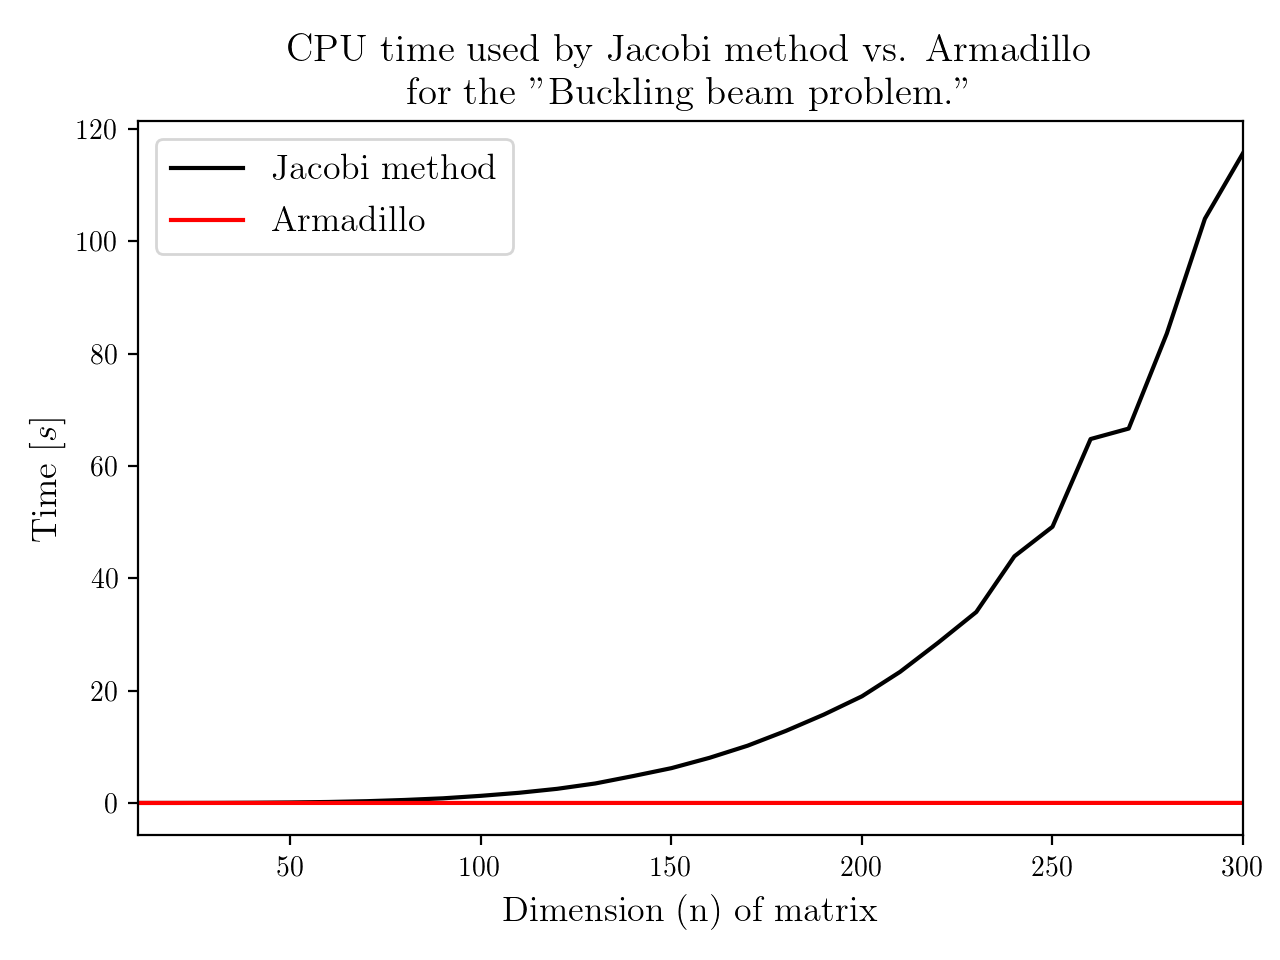
\includegraphics[scale= 0.75]{Figure_1_Project_2.png}}
\caption{Comparison of the CPU time for Jacobi's method and Armadillo's\cite{Sanderson2019}\cite{Saddler1971} built-in solver for eigenvalue problems $eig\_sym$ to diagonalize the Toeplitz matrix to a diagonal matrix, for the "Buckling beam problem".}
\label{fig:CPU}
\end{figure}

\begin{figure}[H]
\centerline{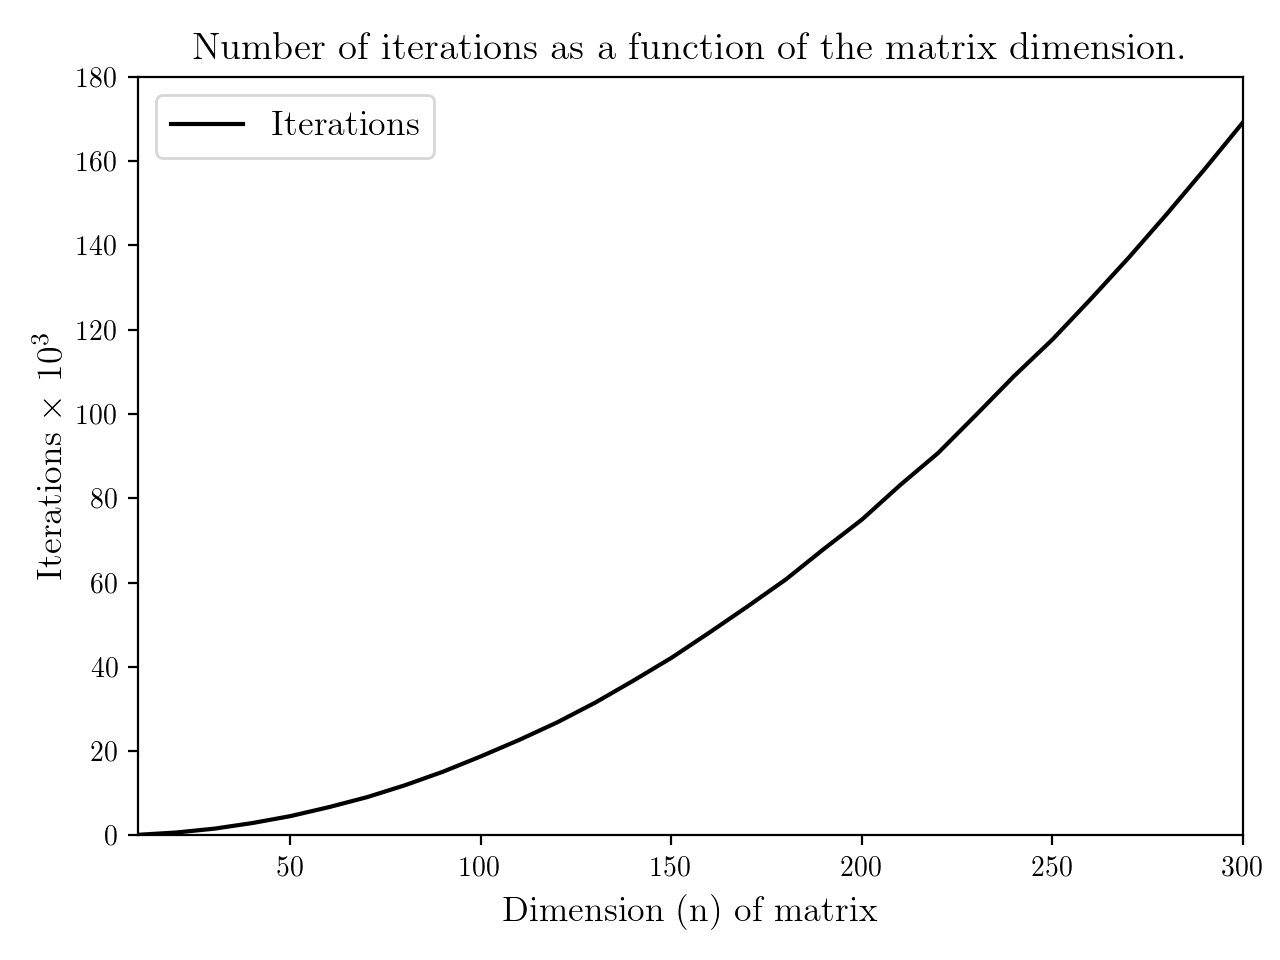
\includegraphics[scale= 0.75]{Figure_2_Project_2.png}}
\caption{Amount of iterations needed to diagonalize the Toeplitz matrix in "Buckling beam problem" as a function of dimension (n) of the matrix with the tolerance for non-diagonal elements set to $\varepsilon = 10^{-10}$.}
\label{fig:Iterations}
\end{figure}

%Figure \ref{fig:CPU} represents the time it takes for Jacobi's method and Armadillo's function $eigsym$ to diagonalize the Toeplitz matrix to a diagonal matrix $\bm{B}.$

\begin{table}[H]
\centering
\caption{Comparing execution time $\&$ number of iterations for the buckling beam problem with altering dimension N. Values from this table are extracted from \textcolor{red}{\href{https://github.com/patrykpk/FYS4150/tree/master/Project_2}{GitHub}} under the folder "Results/Buckling{\_}beam".}
\label{tab:buckling_beam}
\begin{tabular}{|c|c|c|c|c|}
\hline
\multicolumn{5}{|c|}{\textit{\textbf{Execution time  $\&$ Number of iteration }}} \\ \hline
N & \textit{Jacobi method [s]} & \textit{Armadillo [s]} & Number of iterations & Iterations in $N^2$ \\ \hline
50 & 0.088551 & 0.000213 & 4589 & $1.84N^2$   \\ \hline
100 & 1.270201 & 0.001131 & 18773 & $1.88N^2$    \\ \hline
150 & 6.1998370 & 0.002375 & 42140 & $1.87N^2$   \\ \hline
200 & 18.991274 & 0.004293 & 74944 & $1.87N^2$ \\ \hline
250 & 49.172810 & 0.007059 & 117655 & $1.88N^2$    \\ \hline
300 & 115.68532 & 0.010477 & 169180 & $1.88N^2$  \\ \hline
\end{tabular}
\end{table}

%Skal vi skrive [s] på slutten av alle tidene i Jacobi og Armadillo? Skreiv d bare på rad to, "Bra med rad 2 bare!-Marius"

Information seen in Table \ref{tab:buckling_beam} represents values that have been visualized by Figure \ref{fig:CPU} and Figure \ref{fig:Iterations} and shows some interesting numbers related to the buckling beam. Table \ref{tab:buckling_beam} is only ran over a few N, from 50 to 300N's with a spacing of 50N. Values seen from this table are done with tolerance for the off-diagonal elements set to $\varepsilon=10^{-10}$. The vast time-consuming difference in between the Jacobi method and the solver from Armadillo is discussed in the upcoming section. The number of iterations as a function of matrix dimension N is also included in table \ref{tab:buckling_beam}, in addition the dimensionality was extracted from the iterations to represent the behaviour in a clearer form.


\subsection{Numerical analysis of Quantum dots for one and two electrons}
Adding the harmonic oscillator potential required finding an appropriate approximation to infinity for $\rho_{max}$. This was done by trial and error, and the results given in this section include that one value of $\rho_{max} = 5.5$ that was found. \\

\begin{figure}[H]
\hspace{-1.0in}
     \subfloat[][Part of the results showing the absolute error between the four lowest \\
    analytical and computed eigenvalues from N=10 to N=100.]{ {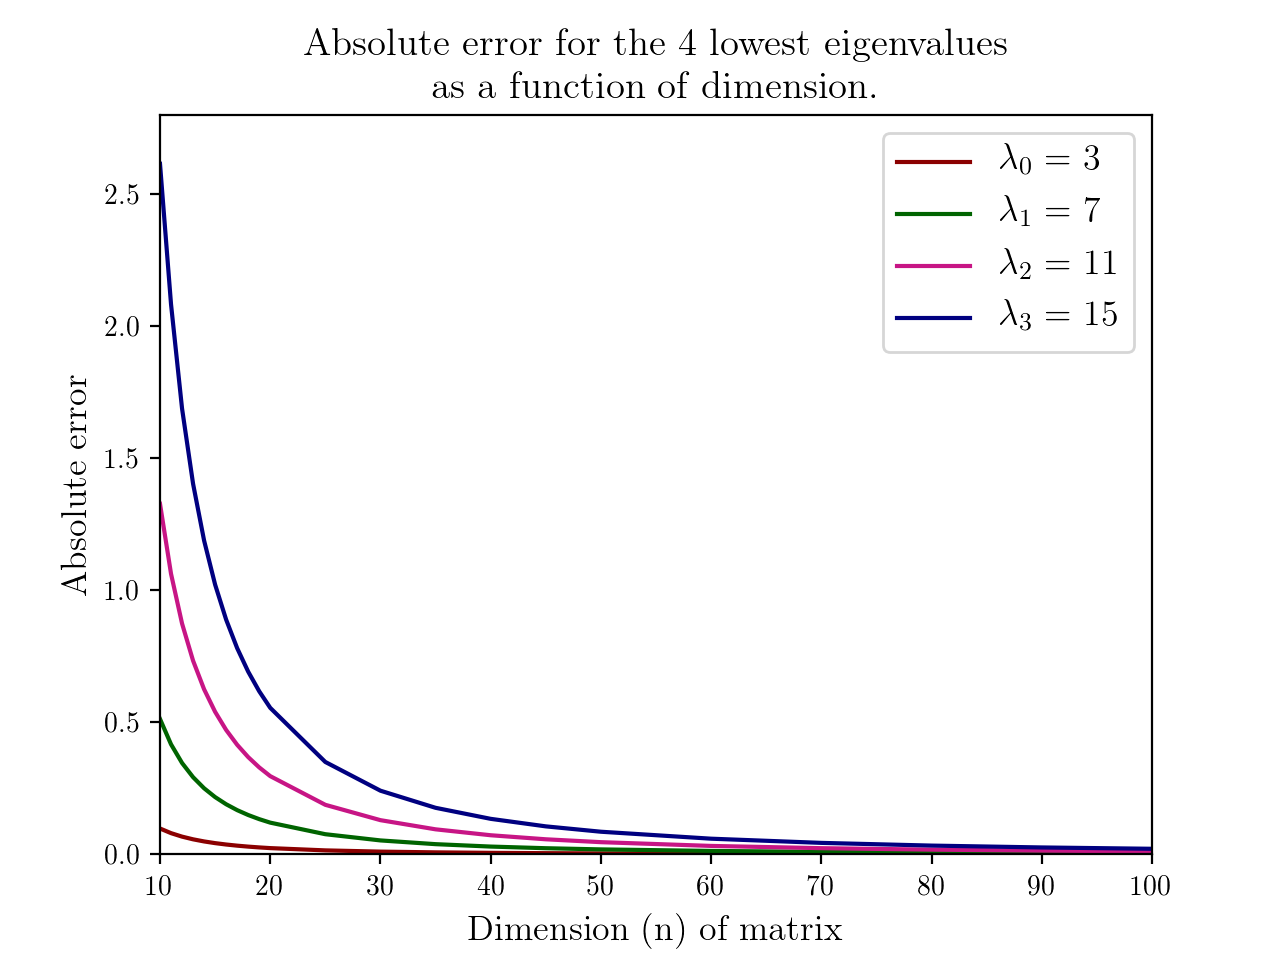
\includegraphics[scale = 0.62]{Figure_3_Project_2.png}}}
     \subfloat[][Part of the results showing the dimension of the matrix where the four lowest energy eigenvalues are below the threshold for deviation of $10^{-3}$.]{{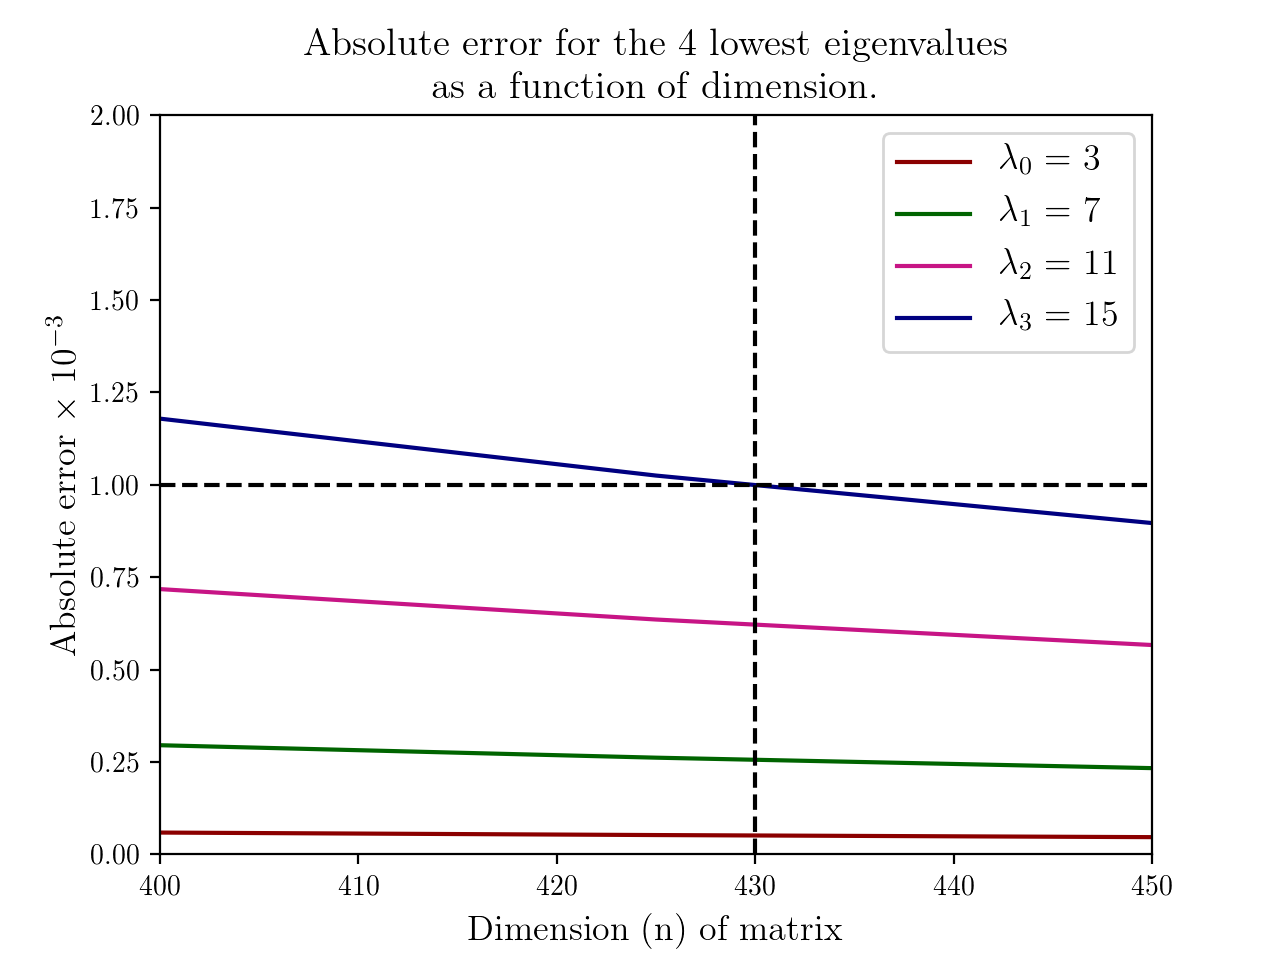
\includegraphics[scale = 0.62]{Figure_4_Project_2.png}}}
       \caption{Absolute error for the four lowest energy eigenvalues as a function of dimension for two different sections with $\rho_{max}=5.5$ (a)  between N=10 to N=100 and (b) between N = 400 and N=450.}
     \label{fig:Eigenvalues}
\end{figure}



Figure \ref{fig:Eigenvalues} shows how the absolute error between the analytical eigenvalues and computed eigenvalues changes as a function of the dimensionality of the matrix. Acquiring high precision with three leading digits accuracy to the analytical results is given by the horizontal line. The value of N where all the eigenvalues have the desired precision can be seen from Figure \ref{fig:Eigenvalues} (b) .

\bigskip
%The most interesting values from Figure \ref{fig:Eigenvalues} are also included in Table \label{tab:qdot1}.
In Table \ref{tab:qdot1} we have found for which N the absolute error is less than $10^{-3}$. In comparison with Figure \ref{fig:Eigenvalues}, we can see that in order to achieve the desired precision of $10^{-3}$ for all eigenvalues, we must increase our matrix dimension to N = 430. The necessary dimension for eigenvalues $\lambda_0,\lambda_1$ and $\lambda_2$ are also included in Table \ref{tab:qdot1}.

\begin{table}[H]
\centering
\caption{Dimension of the matrix where the four lowest energy eigenvalues have acquired the desired precision of $10^{-3}$ from the analytical results. Analytic and numerical results are added to the table as well as absolute error with $\rho_{max} = 5.5$. Values from this table are extracted from \textcolor{red}{\href{https://github.com/patrykpk/FYS4150/tree/master/Project_2}{GitHub}} under the folder "Results/Qdot1".}
\label{tab:qdot1}
\begin{tabular}{|c|c|c|c|c|}
\hline
\multicolumn{5}{|c|}{\textit{\textbf{Three leading digits deviation from the analytical results}}}    \\ \hline
\textit{N} & \textit{Eigenvalue} & \textit{Analytical} & \textit{Numerical} & \textit{Absolute Error} \\ \hline
    98     &        $\lambda_0$         &   3                   &   2.9990154                 &        $9.846\times10^{-4}$                 \\ \hline
    218     &        $\lambda_1$         &   7                   &     6.9990053               &      $9.947\times 10^{-4}$                   \\ \hline
    340     &        $\lambda_2$         &  11                   &     10.999005               &      $9.948\times 10^{-4}$                   \\ \hline
    430     &        $\lambda_3$         &  15                   &    14.999002                &       $9.976\times 10^{-4}$                  \\ \hline
\end{tabular}
\end{table}

For the two-electron system, we implemented a coulomb potential as well as $\omega_r$. Results represented for this system is obtained with various $\omega_r$: 


\begin{table}[H]
	\hspace{-0.9cm}\begin{minipage}{0.5\linewidth}
		\centering
		\vspace{-0.15\textwidth}
		\captionsetup{skip=10pt, width=1.0\linewidth}
		\caption{Table showing the different groundstate \\ 
				eigenvalues for different $\omega_r$. Parameter $N$ and \\ 
				$\rho_{max}$ set to 500 and 30 respectively. Groundstate\\
				eigenvalues with corresponding $\omega_r$. Values from\\
				 this table are extracted from \textcolor{red}{\href{https://github.com/patrykpk/FYS4150/tree/master/Project_2}{GitHub}} under\\ 
				 the folder "Results/Qdot2".}
		\label{tab:Qdot2}
		\begin{tabular}{|c|c|}
			\hline
			\multicolumn{2}{|c|}{\textit{\textbf{Groundstate eigenvalue as a function of $\omega_r$.}}} \\ \hline
			$\omega_r$ & \textit{Eigenvalue}  \\ \hline
			0.01 & 0.10861300   \\ \hline
			0.50 & 2.2298316   \\ \hline
			1.00 & 4.0566975   \\ \hline
			2.00 & 7.5184786 \\ \hline
			3.00 & 10.870268 \\ \hline
			4.00 & 14.163794  \\ \hline
			5.00 & 17.419189 \\ \hline
		\end{tabular}
	\end{minipage}\hfill
	\begin{minipage}{0.6\linewidth}
		\vspace{0.2\textwidth}
		\centering
		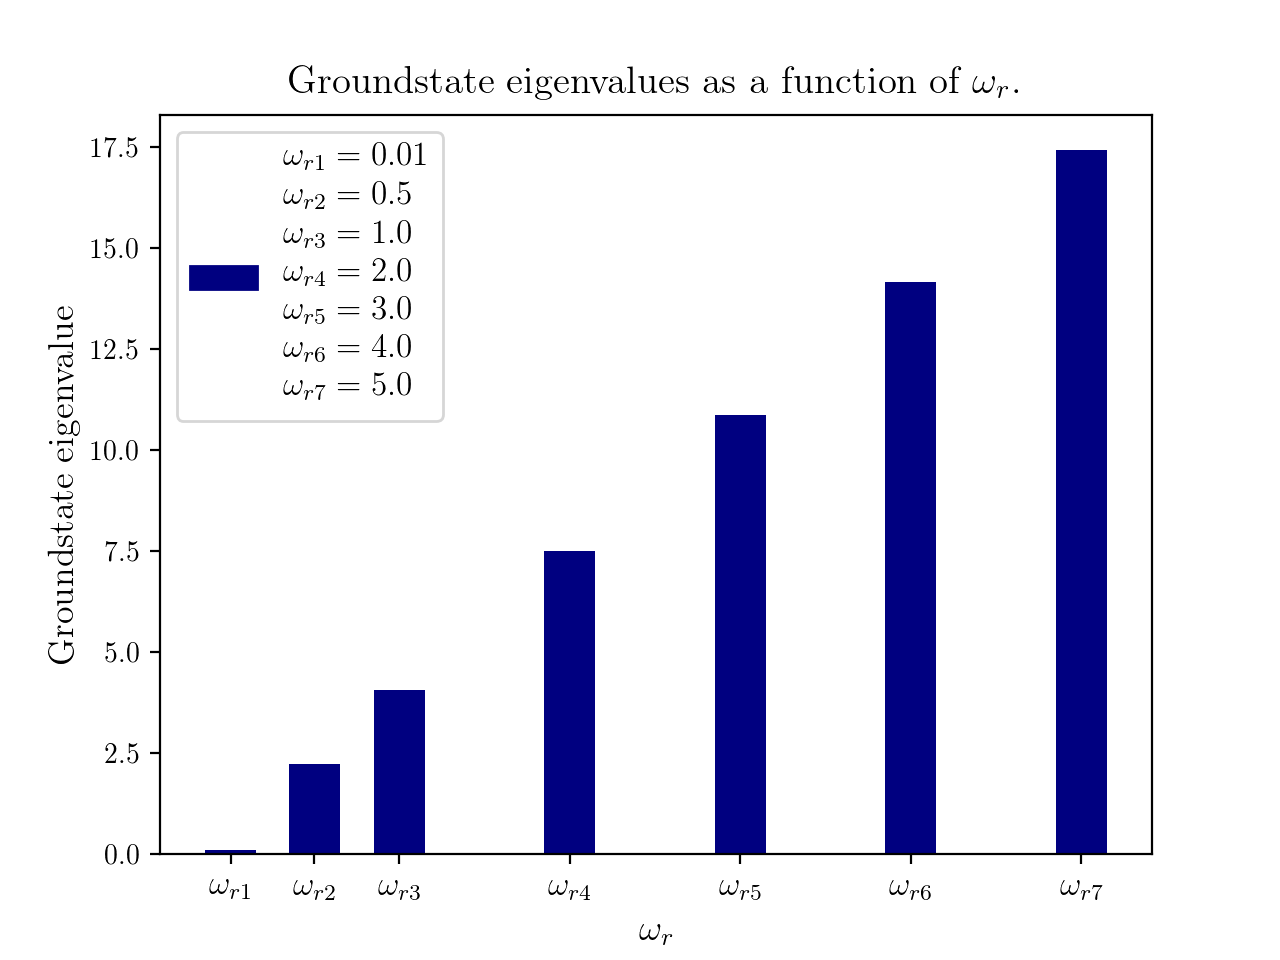
\includegraphics[scale = 0.65]{Figure_5_Project_2.png}
		\captionof{figure}{\leftskip=7em Plot of the data from table 3.}
		\label{fig:Groundstate eigenvalue}
	\end{minipage}
\end{table}

%Footnote under footer
\newcommand{\fancyfootnotetext}[2]{%
  \fancypagestyle{dingens}{%
    \fancyfoot{} % Blank out the default footer
    \fancyfoot[L]{\footnotemark[#1]\footnotesize #2}%
    \fancyfoot[R]{\thepage} 
  }%
  \thispagestyle{dingens}%
}


Figure \ref{fig:Groundstate eigenvalue} shows how the ground state eigenvalue varies with increasing $\omega_{r}$. We can clearly see that by increasing the diagonal elements\footnotemark[1]\fancyfootnotetext{1}{The diagonal element for the two electron case is expressed as $d_i = \frac{2}{h^2} + \omega_r^2\rho_i^2 + \frac{1}{\rho_i}$} in our tridiagonal Toeplitz matrix we get higher values of the ground state eigenvalues. 


%----------------------------------------------------------------------------------------------------------------
%                                                DISCUSION
%----------------------------------------------------------------------------------------------------------------
\newpage

\section{Discussion}

\noindent From Table 1, we clearly see that Armadillo's \textit{eig\_sym}-function (\cite{Sanderson2019} \cite{Saddler1971}) outperforms our implementation of Jacobi's rotation algorithm with respect to CPU time. For $n=50$ the difference in CPU time between Armadillo and Jacobi is over two orders of magnitude. And for $n \geq 100$ the difference in CPU time becomes over three orders of magnitude. \\

This is no surprise, considering the poor convergence rate of the Jacobi method, where one needs typically $3n^2$ - $5n^2$ rotations and each rotation requires $4n$ operations, resulting in $12n^3$ - $20n^3$ operations in order to zero out non-diagonal matrix elements\cite{Morten}. The consideration of number of flops is vital when analysing CPU-time, another way of looking at this is by understanding for which matrix the Jacobi method is designed for. Evaluating the Armadillo \textit{eig\_sym} with Jacobi's method we see that \textit{eig\_sym} is a better way to go about. We need to keep in mind that we are working with a trigional Toeplitz matrix, which has special properties. Then Armadillo's \textit{eig\_sym}-function is probably a more efficient algorithm for finding eigenvalues of tridiagonal matrices. 

\bigskip

%In addition, by extrapolating further from Table 1 we see that there is a relation between the dimension of the matrix and the number of iterations needed for computation in the Jacobi's rotation algorithm. This could have an impact when considering the CPU time needed for the Jacobi's method. \\


Table \ref{tab:qdot1} gives us the numerical eigenvalues for the case of quantum dot with one electron. The numerical results are close to the analytical ones ($\lambda =\ 3,\ 7,\ 11,\ 15,\ \dots$), but reproducing the analytical results with four leading digits after the decimal point proofs to be difficult using Jacobi's rotation algorithm. As we can see from the results, the CPU-time exhibits an exponential behaviour as a function of dimension N. By this it becomes fairly difficult to obtain a lower absolute error than $10^{-3}$.  

\bigskip

In the quantum dot case with two electrons, we see that the eigenvalues for the ground state increases with increasing $\omega_r$ and constant $\rho_{max}$. This makes sense, since a stronger harmonic oscillator potential should lead to higher energies. The value for $\rho_{max}$ was determined by comparing our results with the results of M. Taut\cite{taut}, where a $\rho_{max}\approx30$ was needed for good precision for $\omega_r\approx0.01$. For such a high $\rho_{max}$, the dimension $N$ of the matrix had to be sufficiently high to get sufficient accuracy for higher $\omega_r$, which led to running Jacobi's method with $N=500$ \& $\rho_{max}=30$ for the different values of $\omega_r$.\\


%----------------------------------------------------------------------------------------------------------------
%                                               CONCLUSION
%----------------------------------------------------------------------------------------------------------------

\section{Conclusion}


To conclude the Jacobi's method is a reliable method which offer a neat way to solve eigenvalue problems, however the method is slow for high values of dimension $N$. The results showed clearly that the time exhibited an exponential behaviour as a function of $N$. The special properties of a tridiagonal Toeplitz matrix did not fully take advantage of the Jacobi method. By simplifying our algorithm to only operate on the upper diagonals, we reduced the number of flops by a factor of two.\\

Evaluating the eigenvalue problem for the one electron case showed us that the eigenvalues [$\lambda_0, \lambda_1, \lambda_2, \lambda_3$], was possible to calculate analytically with a high precision set to $10^{-3}$. Higher precision is possible for higher $N$. By trial and error we found out that the value $\rho_{max} = 5.5$, gave the best analytical results. Setting the dimension $N = 430$ we where able to find the eigenvalue of the first five states with an absolute error of $10^{-3}$.\\

Implementing two electrons into our model we found that the eigenvalues of the ground state increased with increasing $\omega_{r}$. As we mentioned in the discussion, a stronger harmonic potential leads to higher energies, as one should expect. Our $\rho_{max}$ where altered in comparison with M.Taut \cite{taut}. Increasing $\rho_{max}$ led us to increase the matrix dimension to keep the desired precision for the given $\omega_r$. 

%----------------------------------------------------------------------------------------
%	REFERENCE LIST
%----------------------------------------------------------------------------------------

\bibliographystyle{unsrt}
\bibliography{Project2_FYS4150}


% ------------------- end of main content ---------------

\end{document}